\documentclass[../main/main.tex]{subfiles}


\begin{document}

\section{February 10th, 2021}
\subsection{Research Methods}
We will cover two different research methods:
\begin{itemize}
  \item Descriptive Research - we only observe/study the relation of the two variables
        \item Experimental Research - we actively manipulate one variable to discover the causal relation between two variables
\end{itemize}
\subsection{Descriptive Research - Case Study}
\index{case study}
\begin{definition}
For a \vocab{case study}, we are investigating an individual or a small group of people intensely.

\end{definition}

\begin{example}
One example of a case study is that of Genie, the feral child.
\end{example}
Case studies have different advantages and disadvantages.
\subsubsection{Advantages}
\begin{itemize}
        \item One key advantage is that we can go deep in investigating the subjects
\item
Case studies are very flexible, as we can tailor the study or alter the research mid way though.
\begin{remark}
Unlike surveys, we can change/alter the research focus during the research process.
\end{remark}

\begin{example}
For example, initially the researchers were investigating Ginnie's language skills. However, through the research process, they found that her understanding is fundamentally different, and as such, they are interested in how she percieves information.
\end{example}
\end{itemize}

\subsubsection{Disadvantages}

\begin{itemize}
\item
The results of a case study might not be generalizable to the general population, as it is specifically focusing on a small group of people.
  \item In a case study, we cannot establish cause and effect.
        \begin{example}
In the case of Ginnie, we don't know if her inability to aquire normal language from here lack of interaction during the critical period, or due to her tramatic experience.
        \end{example}
\end{itemize}

\subsection{Naturalistic Observation}
\begin{definition}
  \index{naturalistic observation}
\vocab{Naturalistic observation} is research in which an investigator simply observes some naturally occurring behavior and does not make a change in the situation.
\end{definition}

\begin{remark}
Naturalistic observation can only be used to observe behaviors, and as such, is not suitable for certain research studies.
\end{remark}
\begin{example}
We can count the number of times students call out or leave their seats at different ages. There is minimal control over the natural environment. Rather the researcher is just observing the students. See Figure \ref{fig:2-10-nat}.
\end{example}
\begin{figure}[htpb]
  \centering
  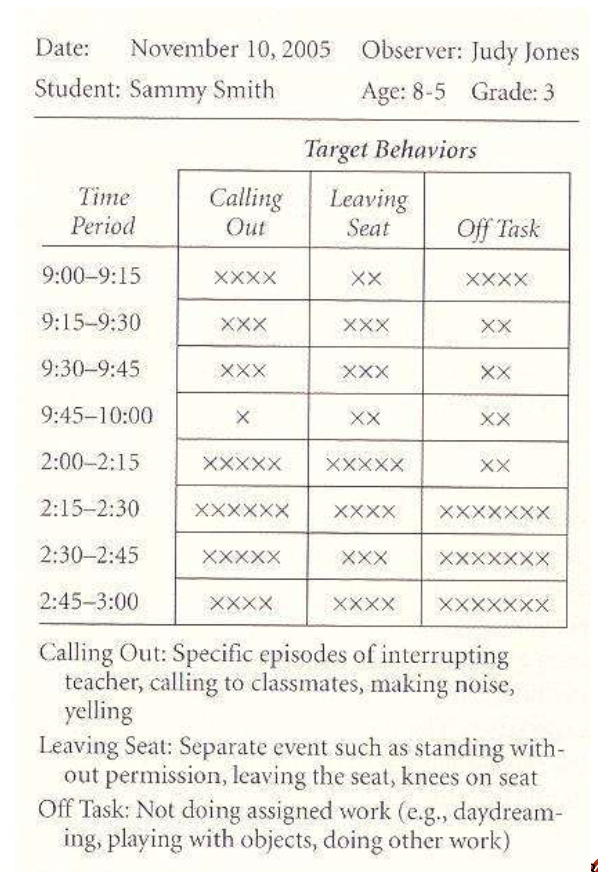
\includegraphics[width=0.5\textwidth]{2-10-nat}
  \caption{Observer sheet for a study examining the relationship between age and behavioral problems}
  \label{fig:2-10-nat}
\end{figure}

When conducting a naturalistic observation, we must consider the following things:

\begin{itemize}
\item We must conduct the study objectively. To do this, we must create an observation chart, which calculates/assess the frequency of behaviors.
        \item We must standardize/define each of the target behaviors.
        \begin{example}
          In the example above, we can define calling out as: specific episodes of interrupting teacher, calling to classmates, making noise, or yelling.
        \end{example}
        This will ensure that the study is conducted objectively.
\end{itemize}

Besides this, we must also consider the following:
\begin{itemize}
  \item Who and how many people are observing?
        \begin{remark}
Using multiple raters will provide more objective results, as there will be less bias. In addition, we can check for \vocab{inter-rater reliability/consistency}. If we find inconsistency in different ratings, we have to figure out why, e.g. some might be more extreme, or the instruction might not be clear.
\index{inter-rater reliability}
        \end{remark}
        If multiple raters have the same results, then we can be more confident that we are capturing the behavior.
        \begin{remark}
We might have to reconduct the study until the results align.
        \end{remark}
  \item Is the study double blind?
        \begin{definition}
Both the participants and the observers must not know the research objective, i.e. the study have a \vocab{double blind design}.
\index{double blind}
        \end{definition}
        \begin{remark}
          Studies must be double blind to ensure that the participants and the rater do not know the purpose of the study, as that would affect their actions/evaluations.
        \end{remark}
\end{itemize}
\subsubsection{Advantages}
The results of naturalistic observation can usually be generalized to the general population, as people are assumed to behave naturally in their natural environment.
\begin{remark}
This is different from experimental study, where the context or design of the study might be very different from real life.
\end{remark}

\subsubsection{Disadvantages}
\begin{itemize}
\item If people know that they are being observed, the participants might deliberately change their behaviors
        \begin{example}
If we are studying parent-child interactions and the parents know this, they might change their interactions
        \end{example}
        \begin{remark}
Sometimes we want to disguise the observation. However, this is not always the case, as we might need consent from the participants.
        \end{remark}
  \item No causal relationships can be drawn.
\begin{example}
In the example, the observations change based on time, with the students displaying more behavior problems in the afternoon. Thus, we might speculate that students' attention span decrease over time. However, this hypothesis cannot be verified from this study.
\end{example}
  \item Observer bias.
        \begin{definition}
When observing the participants, the observer might have certain bias that will affect their
        \end{definition}
        \begin{example}
In the example before, observers might think that older students are more well behaved, but this will affect how they perceive the students.
        \end{example}
\begin{remark}
In order to minimize observer bias, we use multiple observers and a double blind study.
\end{remark}
\end{itemize}


\subsection{Descriptive Research - Correlational Study}
\begin{definition}\vocab{Correlational study} is research in which the relationship between two variables is examined to determine whether they are associated or correlated
  \index{correlational study}
\end{definition}
\begin{example}
  Some variables that can be the subject of correlational study include:
\begin{itemize}
\item Age and self-esteem
  \item High school grades and university GPA
        \item Time playing on the internet and social network
\end{itemize}
\end{example}
In a correlational study, there are two objectives:
\begin{enumerate}
  \item Determine the direction of association among variables
        \begin{remark}
Whether the two variables are positively or negatively correlated. Positive means they increase together, while negative is opposite.
        \end{remark}
  \item Examine the magnitude of association among variables
        \begin{remark}
Correlation varies from -1 to 1. The higher the absolute value of correlation, the more they are correlated.
        \end{remark}
\end{enumerate}
When designing a correlational study, we must make sure that the variables are quantifiable numerically.
\begin{definition}
In order to be used in a correlational study, we must have an \vocab{operational definition} of the variable.
\index{operational definition}
\end{definition}
\begin{remark}
The operational definition might change from study to study. For example, if we want to measure the use of internet, we might use hrs/week, or we might investigate more specific usage, e.g. number of time checking social media per day.
\end{remark}
The general rule of thumb is if the magnitude of correlation is:
\begin{itemize}
  \item $< 0.3$: the correlation is weak
  \item $> 0.3$ and $< 0.7$: the correlation is moderate
        \item $>0.7$: the correlation is strong
\end{itemize}

\begin{remark}
Even if the correlation is 0, we cannot say that there is no correlation. The relationship might be non linear. See Figure \ref{2-10-corr}. If the relationship is non-linear, the correlation coefficient cannot capture the relation. Make sure to not jump to conclusion if it is zero.
\end{remark}
\begin{figure}[htpb]
  \centering
  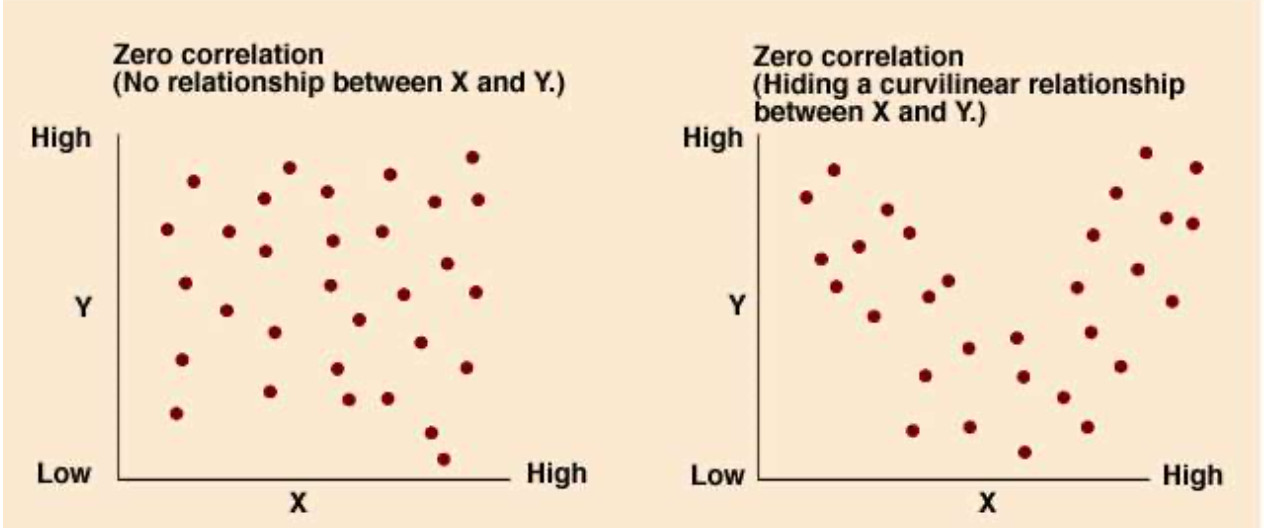
\includegraphics[width=0.8\textwidth]{2-10-corr}
  \caption{Non-linear correlation, but both have a correlation coefficient of 0}
  \label{2-10-corr}
\end{figure}
One thing we have to note is that correlation does not imply a causal relationship.
\begin{example}
  \label{2-10-corr-ex}
  Imaging you found a correlation (R = -0.6) between time playing on the internet and the number of friends. However, there are a few different interpretations, as can be seen in Figure \ref{2-10-friends}.
\end{example}
  \begin{figure}[htpb]
	\centering
	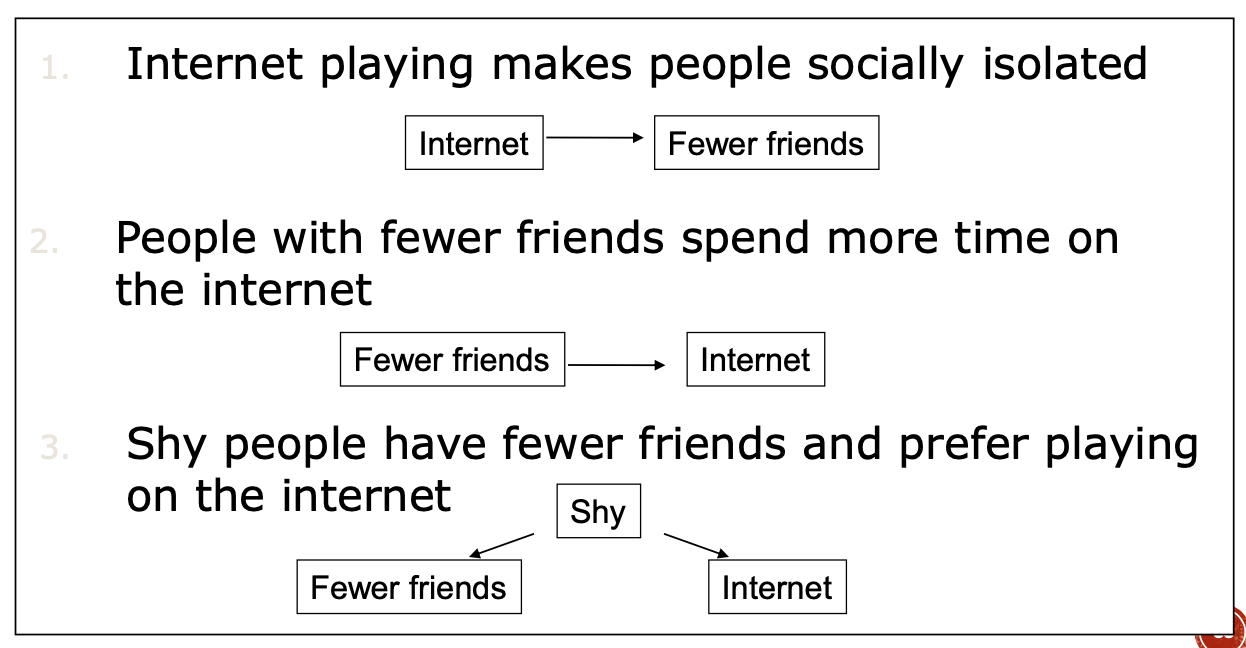
\includegraphics[width=0.7\textwidth]{2-10-friends}
	\caption{Different ways to interpret the correlation}
	\label{2-10-friends}
  \end{figure}
\begin{definition}
In Example \ref{2-10-corr-ex}, shyness is a \vocab{confounding variable}.
\index{confounding variable}
\end{definition}
\begin{remark}
In Example \ref{2-10-corr-ex}, the correlation is moderately negative.
\end{remark}
\begin{example}
  Other examples of interpreting correlations:
  \begin{itemize}
    \item r=0.5 between show size and vocabulary size. Age is a confounding variable
          \item r=0.55 between number of bottled water and healthier babies. Family income is a confounding variable.
          \item r=0.4 between number of fire engines and amount of damage. More damage requires more fire engines.
  \end{itemize}
\end{example}
There are a few takeaways from correlational studies:
\begin{itemize}
        \item There are three possible interpretation of correlation
\item Even if there is a correlation, the variables might not be related. It could be a confounding variable.
\end{itemize}
\subsection{Experimental Research}
\begin{definition}
  \vocab{Experimental research} is research in which we deliberate vary one variable and observe the change in another.
  \index{experimental research}
\end{definition}
There are two types of variables in experimental research:
\begin{itemize}
  \item \vocab{Independent variable (IV)} - the variable that is being changed
        \index{independent variable}
        \item \vocab{Dependent variable (DV)} - the variable that is being observed
        \index{dependent variable}
\end{itemize}
\begin{example}
  Consider a study where we want to see the relationship of viewing violent TV and the physical aggression of people. In this case, the variables are:
  \begin{itemize}
          \label{2-10-vio}
    \item IV: Violent TV
          \item DV: Number of physical fights when playing with friends
  \end{itemize}
\end{example}
In order to carry out the study, we must recruit participants. There must be two conditions:
\begin{enumerate}
  \item Experimental Condition - Change the IV
        \item Control Condition - Do not change the IV
\end{enumerate}
\begin{example}
For Example \ref{2-10-vio}, the experimental condition would be exposed to violent TV, while the control group is exposed to non-violent TV.
\end{example}

\begin{remark}
The control group is important, as it serves as the comparison group. We will see the difference between people who are exposed to the change in IV.
\end{remark}
The core logic is that we must ensure that the two groups are identical in all aspect except for the IV. This way we can be sure that the change in the DV is because of the change in the IV.

\begin{example}
  If in Example \ref{2-10-vio}, if the experimental group was mostly male, but the control group was mostly female, and the experimental group was found to be more physically violent. It could be because they are exposed to violent TV, but it could also be because men are naturally more physical than women.
\end{example}

\end{document}
